% Created 2022-11-04 Fri 14:56
% Intended LaTeX compiler: pdflatex
\documentclass[11pt]{article}
\usepackage[utf8]{inputenc}
\usepackage[T1]{fontenc}
\usepackage{graphicx}
\usepackage{longtable}
\usepackage{wrapfig}
\usepackage{rotating}
\usepackage[normalem]{ulem}
\usepackage{amsmath}
\usepackage{amssymb}
\usepackage{capt-of}
\usepackage{hyperref}
\graphicspath{{../../books/}}
% TIPS
% \substack{a\\b} for multiple lines text





% pdfplots will load xolor automatically without option
\usepackage[dvipsnames]{xcolor}

\usepackage{forest}
% two-line text in node by [two \\ lines]
% \begin{forest} qtree, [..] \end{forest}
\forestset{
  qtree/.style={
    baseline,
    for tree={
      parent anchor=south,
      child anchor=north,
      align=center,
      inner sep=1pt,
    }}}
%\usepackage{flexisym}
% load order of mathtools and mathabx, otherwise conflict overbrace

\usepackage{mathtools}
%\usepackage{fourier}
\usepackage{pgfplots}
\usepackage{amsthm, mathabx,  amsmath, commath}
\usepackage{amsfonts}

\usepackage{empheq}
\usepackage{tikz}
\usetikzlibrary{arrows.meta}
\usepackage[most]{tcolorbox}

\newtheorem{theorem}{Theorem}[section]
\newtheorem{definition}{Definition}[section]
\newtheorem{corollary}{Corollary}[section]
\newtheorem{example}{Example}[section]
\newtheorem{lemma}{Lemma}[section]
\newtheorem{proposition}{Proposition}[section]

\newcommand{\bl}[1] {\boldsymbol{#1}}
\newcommand{\Wt}[1] {\stackrel{\sim}{\smash{#1}\rule{0pt}{1.1ex}}}
\newcommand{\wt}[1] {\widetilde{#1}}


%For boxed texts in align, use Aboxed{}
%otherwise use boxed{}

\DeclareMathSymbol{\widehatsym}{\mathord}{largesymbols}{"62}
\newcommand\lowerwidehatsym{%
  \text{\smash{\raisebox{-1.3ex}{%
    $\widehatsym$}}}}
\newcommand\fixwidehat[1]{%
  \mathchoice
    {\accentset{\displaystyle\lowerwidehatsym}{#1}}
    {\accentset{\textstyle\lowerwidehatsym}{#1}}
    {\accentset{\scriptstyle\lowerwidehatsym}{#1}}
    {\accentset{\scriptscriptstyle\lowerwidehatsym}{#1}}
}

\usepackage{graphicx}
    
% text on arrow for xRightarrow
\makeatletter
%\newcommand{\xRightarrow}[2][]{\ext@arrow 0359\Rightarrowfill@{#1}{#2}}
\makeatother


\def \bx {\boldsymbol{x}}
\def \ba {\boldsymbol{a}}
\def \bI {\boldsymbol{I}}
\def \bt {\boldsymbol{t}}
\def \bb {\boldsymbol{b}}
\def \bA {\boldsymbol{A}}
\def \bX {\boldsymbol{X}}
\def \bu {\boldsymbol{u}}
\def \bS {\boldsymbol{S}}
\def \bZ {\boldsymbol{Z}}
\def \bz {\boldsymbol{z}}
\def \by {\boldsymbol{y}}
\def \bw {\boldsymbol{w}}
\def \bT {\boldsymbol{T}}
\def \bS {\boldsymbol{S}}
\def \bm {\boldsymbol{m}}
\def \bW {\boldsymbol{W}}
\def \bY {\boldsymbol{Y}}
\def \bH {\boldsymbol{H}}
\def \blambda {\boldsymbol{\lambda}}
\def \bPhi {\boldsymbol{\Phi}}
\def \btheta {\boldsymbol{\theta}}
\def \bmu {\boldsymbol{\mu}}
\def \bphi {\boldsymbol{\phi}}
\def \bSigma {\boldsymbol{\Sigma}}
\def \lb {\left\{}
\def \rb {\right\}}
\def \caln {\mathcal{N}}
\def \dissum {\displaystyle\Sigma}
\def \dispro {\displaystyle\prod}
\def \E {\mathbb{E}}
\def \Q {\mathbb{Q}}
\def \V {\mathbb{V}}
\def \R {\mathbb{R}}
\def \calq {\mathcal{Q}}
\def \calg {\mathcal{G}}
\def \caln {\mathcal{N}}
\def \calr {\mathcal{R}}
\def \calm {\mathcal{M}}
\def \calc {\mathcal{C}}
\def \bcup {\bigcup}

\usepackage{minted}
\setminted{fontsize=\footnotesize,baselinestretch=1}
\makeindex
\let\OldTexttt\texttt
\renewcommand{\texttt}[1]{\OldTexttt{\color{MidnightBlue} #1}}
\author{NONE}
\date{\today}
\title{The Rust Book}
\hypersetup{
 pdfauthor={NONE},
 pdftitle={The Rust Book},
 pdfkeywords={},
 pdfsubject={},
 pdfcreator={Emacs 28.0.92 (Org mode 9.6)}, 
 pdflang={English}}
\begin{document}

\maketitle
\tableofcontents


\section{Programming a Guessing Game}
\label{sec:orgcabb4a8}
\begin{minted}[]{rust}
use std::io;

fn main() {
    println!("Guess the number!");

    println!("Please input your guess.");

    let mut guess = String::new();

    io::stdin()
        .read_line(&mut guess)
        .expect("Failed to read line");

    println!("You guessed: {guess}");
}
\end{minted}

Result's variants are \texttt{Ok} and \texttt{Err}. The \texttt{Ok} variant indicates the operation was successful, and
inside \texttt{Ok} is the successfully generated value. The \texttt{Err} variant means the operation failed, and
Err contains information about how or why the operation failed.

An instance of \texttt{Result} has an expect method that you can call. If this instance of \texttt{Result} is an
\texttt{Err} value, expect will cause the program to crash and display the message that you passed as an
argument to expect.

If the \texttt{read\_line} method returns an \texttt{Err}, it would likely be the result of an error coming from
the underlying operating system. If this instance of \texttt{Result} is an \texttt{Ok} value, expect will take the
return value that \texttt{Ok} is holding and return just that value to you so you can use it. In this
case, that value is the number of bytes in the user’s input.

If you don’t call \texttt{expect}, the program will compile, but you’ll get a warning:

The \texttt{\{\}} set of curly brackets is a placeholder.

\begin{minted}[]{rust}
let x = 5;
let y = 10;

println!("x = {} and y = {}", x, y);
\end{minted}

A crate is a collection of Rust source code files. The project we’ve been building is a \textbf{binary
crate}, which is an executable. The \texttt{rand} crate is a \textbf{library crate}, which contains code intended
to be used in other programs and can't be executed on its own.

When we include an external dependency, Cargo fetches the latest versions of everything that
dependency needs from the \texttt{registry}, which is a copy of data from \href{https://crates.io/}{Crates.io}. Crates.io is where
people in the Rust ecosystem post their open source Rust projects for others to use.

Cargo has a mechanism that ensures you can rebuild the same artifact every time you or anyone
else builds your code: Cargo will use only the versions of the dependencies you specified until
you indicate otherwise.

When you build a project for the first time, Cargo figures out all the versions of the
dependencies that fit the criteria and then writes them to the \texttt{Cargo.lock} file. When you build
your project in the future, Cargo will see that the \texttt{Cargo.lock} file exists and use the versions
specified there rather than doing all the work of figuring out versions again. This lets you
have a reproducible build automatically.

When you do want to update a crate, Cargo provides the command \texttt{update}, which will ignore the
\texttt{Cargo.lock} file and figure out all the latest versions that fit your specifications in
\texttt{Cargo.toml}.

\begin{minted}[]{rust}
use std::io;
use rand::Rng;

fn main() {
    println!("Guess the number!");

    let secret_number = rand::thread_rng().gen_range(1..=100);

    println!("The secret number is: {secret_number}");

    println!("Please input your guess.");

    let mut guess = String::new();

    io::stdin()
        .read_line(&mut guess)
        .expect("Failed to read line");

    println!("You guessed: {guess}");
}
\end{minted}

\texttt{rand::thread\_rng} function gives us the particular random number generator that we’re going to
use: one that is local to the current thread of execution and seeded by the operating system.
Then we call the \texttt{gen\_range} method on the random number generator. This method is defined by the
\texttt{Rng} trait that we brought into scope with the \texttt{use rand::Rng} statement. The \texttt{gen\_range} method takes
a range expression as an argument and generates a random number in the range. The kind of range
expression we’re using here takes the form \texttt{start..=end} and is inclusive on the lower and upper
bounds, so we need to specify \texttt{1..=100} to request a number between 1 and 100.

\begin{minted}[]{rust}
use rand::Rng;
use std::cmp::Ordering;
use std::io;

fn main() {
    // --snip--

    println!("You guessed: {guess}");

    match guess.cmp(&secret_number) {
        Ordering::Less => println!("Too small!"),
        Ordering::Greater => println!("Too big!"),
        Ordering::Equal => println!("You win!"),
    }
}
\end{minted}

A \texttt{match} expression is made up of \textbf{arms}. An arm consists of a \textbf{pattern} to match against, and the
code that should be run if the value given to \texttt{match} fits that arm’s pattern.

Unless otherwise specified, Rust defaults to an \texttt{i32}.

Ultimately, we want to convert the \texttt{String} the program reads as input into a real number type so
we can compare it numerically to the secret number. We do so by adding this line to the \texttt{main}
function body:
\begin{minted}[]{rust}
let guess: u32 = guess.trim().parse().expect("Please type a number!");
\end{minted}

We create a variable named \texttt{guess}. But wait, doesn’t the program already have a variable named
\texttt{guess}? It does, but helpfully Rust allows us to \textbf{shadow} the previous value of \texttt{guess} with a new
one. This feature is often used when you want to convert a value from one type to another type.

The \texttt{trim} method on a \texttt{String} instance will eliminate any whitespace at the beginning and end,
which we must do to be able to compare the string to the \texttt{u32}, which can only contain numerical
data. The user must press enter to satisfy \texttt{read\_line} and input their guess, which adds a
newline character to the string.

The \texttt{parse} \href{https://doc.rust-lang.org/std/primitive.str.html\#method.parse}{method} on strings converts a string to another type. Here, we use it to convert from
a string to a number. We need to tell Rust the exact number type we want by using \texttt{let guess: u32}.
The colon (\texttt{:}) after guess tells Rust we’ll annotate the variable’s type.

The \texttt{parse} method will only work on characters that can logically be converted into numbers and
so can easily cause errors. Because it might fail, the \texttt{parse} method returns a \texttt{Result} type, much
as the \texttt{read\_line} method does.

The \texttt{loop} keyword creates an infinite loop.

To further refine the game’s behavior, rather than crashing the program when the user inputs a
non-number, let’s make the game ignore a non-number so the user can continue guessing.

\begin{minted}[]{rust}
let guess: u32 = match guess.trim().parse() {
    Ok(num) => num,
    Err(_) => continue,
};  
\end{minted}

Remember that \texttt{parse} returns a \texttt{Result} type and \texttt{Result} is an enum that has the variants \texttt{Ok} and
\texttt{Err}. We’re using a \texttt{match} expression here, as we did with the \texttt{Ordering} result of the \texttt{cmp}
method.

If \texttt{parse} is able to successfully turn the string into a number, it will return an \texttt{Ok} value
that contains the resulting number. That \texttt{Ok} value will match the first arm’s pattern, and the
\texttt{match} expression will just return the \texttt{num} value that parse produced and put inside the \texttt{Ok}
value. That number will end up right where we want it in the new \texttt{guess} variable we’re
creating.

If \texttt{parse} is \emph{not} able to turn the string into a number, it will return an \texttt{Err} value that
contains more information about the error. The \texttt{Err} value does not match the \texttt{Ok(num)} pattern in
the first match arm, but it does match the \texttt{Err(\_)} pattern in the second arm. The underscore,
\texttt{\_}, is a catchall value; in this example, we’re saying we want to match all \texttt{Err} values, no
matter what information they have inside them. So the program will execute the second arm’s
code, \texttt{continue}, which tells the program to go to the next iteration of the loop and ask for
another guess. So, effectively, the program ignores all errors that parse might encounter!

\section{Common Programming Concepts}
\label{sec:orgc590b59}
\subsection{Variables and Mutability}
\label{sec:org99cf660}
Like immutable variables, \textbf{constants} are values that are bound to a name and are not allowed to
change, but there are a few differences between constants and variables.

First, you aren’t allowed to use \texttt{mut} with constants. Constants aren’t just immutable by
default—they’re always immutable. You declare constants using the \texttt{const} keyword instead of the
let keyword, and the type of the value must be annotated.

Constants can be declared in any scope, including the global scope, which makes them useful for
values that many parts of code need to know about.

The last difference is that constants may be set only to a constant expression, not the result
of a value that could only be computed at runtime.

Example:
\begin{minted}[]{rust}
const THREE_HOURS_IN_SECONDS: u32 = 60 * 60 * 3;
\end{minted}

Rust’s naming convention for constants is to use all uppercase with underscores between words.
\subsection{Data Types}
\label{sec:org7f10b97}
Keep in mind that Rust is a \textbf{statically typed} language, which means that it must know the types
of all variables at compile time. In cases when many types are possible, we must add a type
annotation.
\begin{itemize}
\item \textbf{Scalar Types}

A \textbf{scalar} type represents a single value. Rust has four primary scalar types: integers,
floating-float numbers, Booleans and characters.
\begin{itemize}
\item \textbf{Integer Types}

\begin{center}
\begin{tabular}{lll}
Length & Signed & Unsigned\\
\hline
8-bit & i8 & u8\\
16-bit & i16 & u16\\
32-bit & i32 & u32\\
64-bit & i64 & u64\\
128-bit & i128 & u128\\
arch & isize & usize\\
\end{tabular}
\end{center}

The \texttt{isize} and \texttt{usize} types depend on the architecture of the computer your program is
running on, which is denoted in the table as “arch”: 64 bits if you’re on a 64-bit
architecture and 32 bits if you’re on a 32-bit architecture.

\begin{center}
\begin{tabular}{ll}
Number Literals & Example\\
\hline
Decimal & 98\textunderscore222\\
Hex & 0xff\\
Octal & 0o77\\
Binary & 0b1111\textunderscore0000\\
Byte(\texttt{u8} only) & b'A'\\
\end{tabular}
\end{center}

When you’re compiling in release mode with the \texttt{-{}-release} flag, Rust does \textbf{not} include checks
for integer overflow that cause panics. Instead, if overflow occurs, Rust performs
\textbf{two’s complement wrapping}. In short, values greater than the maximum value the type can
hold “wrap around” to the minimum of the values the type can hold. In the case of a u8, the
value 256 becomes 0, the value 257 becomes 1, and so on.

To explicitly handle the possibility of overflow, you can use these families of methods
provided by the standard library for primitive numeric types:
\begin{itemize}
\item Wrap in all modes with the \texttt{wrapping\_*} methods, such as \texttt{wrapping\_add}
\item Return the \texttt{None} value if there is overflow with the \texttt{checked\_*} methods
\item Return the value and a boolean indicating whether there was overflow with the
\texttt{overflowing\_*} methods
\item Saturate at the value’s minimum or maximum values with \texttt{saturating\_*} methods
\end{itemize}
\item \textbf{Floating-Point Types}

Rust’s floating-point types are \texttt{f32} and \texttt{f64}, which are 32 bits and 64 bits in size, the
default type is \texttt{f64}. All floating-point types are signed.
\item \textbf{Boolean Type}

The Boolean type in Rust is specified using \texttt{bool}.
\item \textbf{Character Type}

\begin{minted}[]{rust}
fn main() {
    let c = 'z';
    let z: char = 'ℤ'; // with explicit type annotation
    let heart_eyed_cat = '😻';
}
\end{minted}

Rust's \texttt{char} type is four bytes in size and represents a Unicode Scalar Value, which means it
can represent a lot more than ASCII.

Unicode Scalar Values range from \texttt{U+0000} to \texttt{U+D7FF} and \texttt{U+E000} to \texttt{U+10FFFF} inclusive.
\end{itemize}
\item \textbf{Compound Types}
\begin{itemize}
\item \textbf{The Tuple Type}

A tuple is a general way of grouping together a number of values with a variety of types
into one compound type. Tuples have a fixed length: once declared, they cannot grow or
shrink in size.

\begin{minted}[]{rust}
fn main() {
    let tup: (i32, f64, u8) = (500, 6.4, 1);
}
\end{minted}
To get the individual values out of a tuple, we can use pattern matching to destructure a
tuple value, like this:
\begin{minted}[]{rust}
fn main() {
    let tup = (500, 6.4, 1);

    let (x, y, z) = tup;

    println!("The value of y is: {y}");
}
\end{minted}
This is called \textbf{destructuring}, because it breaks the single tuple into three parts.

We can also access a tuple element directly by using a period (\texttt{.}) followed by the index of
the value we want to access. For example:
\begin{minted}[]{rust}
fn main() {
    let x: (i32, f64, u8) = (500, 6.4, 1);

    let five_hundred = x.0;

    let six_point_four = x.1;

    let one = x.2;
}
\end{minted}

The tuple without any values has a special name, \textbf{unit}. This value and its corresponding type
are both written () and represent an empty value or an empty return type. Expressions
implicitly return the unit value if they don’t return any other value.
\item \textbf{The Array Type}

Unlike a tuple, every element of an array must have the same type. Unlike arrays in some
other languages, arrays in Rust have a fixed length.

You write an array’s type using square brackets with the type of each element, a semicolon,
and then the number of elements in the array, like so:
\begin{minted}[]{rust}
let a: [i32; 5] = [1, 2, 3, 4, 5];
\end{minted}

You can also initialize an array to contain the same value for each element by specifying
the initial value, followed by a semicolon, and then the length of the array in square
brackets, as shown here:
\begin{minted}[]{rust}
let a = [3; 5];
\end{minted}

An array is a single chunk of memory of a known, fixed size that can be allocated on the
stack. You can access elements of an array using indexing, like this:
\begin{minted}[]{rust}
fn main() {
    let a = [1, 2, 3, 4, 5];

    let first = a[0];
    let second = a[1];
}
\end{minted}
\end{itemize}
\end{itemize}
\subsection{Functions}
\label{sec:org0118dde}
Rust code uses \textbf{snake case} as the conventional style for function and variable names, in which
all letters are lowercase and underscores separate words.

Rust doesn’t care where you define your functions, only that they’re defined somewhere in a
scope that can be seen by the caller.

\textbf{Statements} are instructions that perform some action and do not return a value. \textbf{Expressions}
evaluate to a resulting value. Let’s look at some examples.

Function definitions are also statements; the entire preceding example is a statement in itself.

Statements do not return values. Therefore, you can’t assign a \texttt{let} statement to another variable.

new scope block created with curly brackets is an expression, for example:
\begin{minted}[]{rust}
fn main() {
    let y = {
        let x = 3;
        x + 1
    };

    println!("The value of y is: {y}");
}
\end{minted}

The expression:
\begin{minted}[]{rust}
{
    let x = 3;
    x + 1
}
\end{minted}
is a block that, in this case, evaluates to \texttt{4}. That value gets bound to \texttt{y} as part of the \texttt{let}
statement. Note that the \texttt{x + 1} line doesn’t have a semicolon at the end, unlike most of the
lines you’ve seen so far. Expressions do not include ending semicolons. If you add a semicolon
to the end of an expression, you turn it into a statement, and it will then not return a value.

Functions can return values to the code that calls them. We don’t name return values, but we
must declare their type after an arrow (\texttt{->}).
\subsection{Control Flow}
\label{sec:orge101602}
\begin{minted}[]{rust}
fn main() {
    let number = 3;

    if number < 5 {
        println!("condition was true");
    } else {
        println!("condition was false");
    }
}
\end{minted}

Because if is an expression, we can use it on the right side of a \texttt{let} statement to assign the
outcome to a variable
\begin{minted}[]{rust}
let number = if condition { 5 } else { 6 };
\end{minted}

One of the uses of a loop is to retry an operation you know might fail, such as checking whether
a thread has completed its job. You might also need to pass the result of that operation out of
the loop to the rest of your code. To do this, you can add the value you want returned after the
break expression you use to stop the loop; that value will be returned out of the loop so you
can use it, as shown here:
\begin{minted}[]{rust}
fn main() {
    let mut counter = 0;

    let result = loop {
        counter += 1;

        if counter == 10 {
            break counter * 2;
        }
    };

    println!("The result is {result}");
}
\end{minted}

If you have loops within loops, \texttt{break} and \texttt{continue} apply to the innermost loop at that point.
You can optionally specify a loop label on a loop that we can then use with \texttt{break} or \texttt{continue} to
specify that those keywords apply to the labeled loop instead of the innermost loop. Loop labels
must begin with a single quote. Here’s an example with two nested loops:

\begin{minted}[]{rust}
fn main() {
    let mut count = 0;
    'counting_up: loop {
        println!("count = {count}");
        let mut remaining = 10;

        loop {
            println!("remaining = {remaining}");
            if remaining == 9 {
                break;
            }
            if count == 2 {
                break 'counting_up;
            }
            remaining -= 1;
        }

        count += 1;
    }
    println!("End count = {count}");
}
\end{minted}

\begin{minted}[]{rust}
fn main() {
    let mut number = 3;

    while number != 0 {
        println!("{number}!");

        number -= 1;
    }

    println!("LIFTOFF!!!");
}
\end{minted}

\begin{minted}[]{rust}
fn main() {
    let a = [10, 20, 30, 40, 50];

    for element in a {
        println!("the value is: {element}");
    }
}

fn main() {
    for number in (1..4).rev() {
        println!("{number}!");
    }
    println!("LIFTOFF!!!");
}
\end{minted}
\section{Understanding Ownership}
\label{sec:org20f700c}
\subsection{What is Ownership?}
\label{sec:orga3008ae}
\textbf{Ownership} is a set of rules that governs how a Rust program manages memory. All programs have to
 manage the way they use a computer's memory while running.

Rust uses a third approach: memory is managed through a system of ownership with a set of rules
that the compiler checks. If any of the rules are violated, the program won’t compile. None of
the features of ownership will slow down your program while it’s running.

The heap is less organized: when you put data on the heap, you request a certain amount of
space. The memory allocator finds an empty spot in the heap that is big enough, marks it as
being in use, and returns a pointer, which is the address of that location. This process is
called \textbf{allocating} on the heap and is sometimes abbreviated as just \textbf{allocating} (pushing values
onto the stack is not considered allocating). Because the pointer to the heap is a known, fixed
size, you can store the pointer on the stack, but when you want the actual data, you must
follow the pointer.

Pushing to the stack is faster than allocating on the heap because the allocator never has to
search for a place to store new data. Accessing data in the heap is slower than accessing data
on the stack because you have to follow a pointer to get there.

Keeping track of what parts of code are using what data on the heap, minimizing the amount of
duplicate data on the heap, and cleaning up unused data on the heap so you don’t run out of
space are all problems that ownership addresses.

\textbf{Ownership Rules}
\begin{itemize}
\item Each value in Rust has an \textbf{owner}.
\item There can only be one owner at a time.
\item When the owner goes out of scope, the value will be dropped.
\end{itemize}

We’ll concentrate on the parts of \texttt{String} that relate to ownership.

You can create a String from a string literal using the from function, like so:
\begin{minted}[]{rust}
let s = String::from("hello");
\end{minted}

This kind of string \textbf{can} be mutated:
\begin{minted}[]{rust}
let mut s = String::from("hello");

s.push_str(", world!"); // push_str() appends a literal to a String

println!("{}", s); // This will print `hello, world!`
\end{minted}

So, what’s the difference here? \textbf{Why can String be mutated but literals cannot?} The difference
is how these two types deal with memory.

In the case of a string literal, we know the contents at compile time, so the text is
hardcoded directly into the final executable. This is why string literals are fast and
efficient. But these properties only come from the string literal’s immutability.

With the String type, in order to support a mutable, growable piece of text, we need to
allocate an amount of memory on the heap, unknown at compile time, to hold the contents. This
means:
\begin{itemize}
\item The memory must be requested from the memory allocator at runtime
\item We need a way of returning memory to the allocator when we're done with our \texttt{String}.
\end{itemize}

That first part is done by us: when we call \texttt{String::from}, its implementation requests the
memory it needs.

However, the second part is different. In languages with a \texttt{garbage collector} (GC), the GC
keeps track of and cleans up memory that isn’t being used anymore, and we don’t need to think
about it. In most languages without a GC, it’s our responsibility to identify when memory is
no longer being used and call code to explicitly free it, just as we did to request it. Doing
this correctly has historically been a difficult programming problem. If we forget, we’ll
waste memory. If we do it too early, we’ll have an invalid variable. If we do it twice, that’s
a bug too. We need to pair exactly one \texttt{allocate} with exactly one \texttt{free}.

Rust takes a different path: the memory is automatically returned once the variable that owns
it goes out of scope.

There is a natural point at which we can return the memory our String needs to the allocator:
when s goes out of scope. When a variable goes out of scope, Rust calls a special function for
us. This function is called \texttt{drop}, and it’s where the author of String can put the code to
return the memory. Rust calls drop automatically at the closing curly bracket.

A String is made up of three parts, shown on the left: a pointer to the memory that holds the
contents of the string, a length, and a capacity. This group of data is stored on the stack.
On the right is the memory on the heap that holds the contents.

\begin{figure}[htbp]
\centering
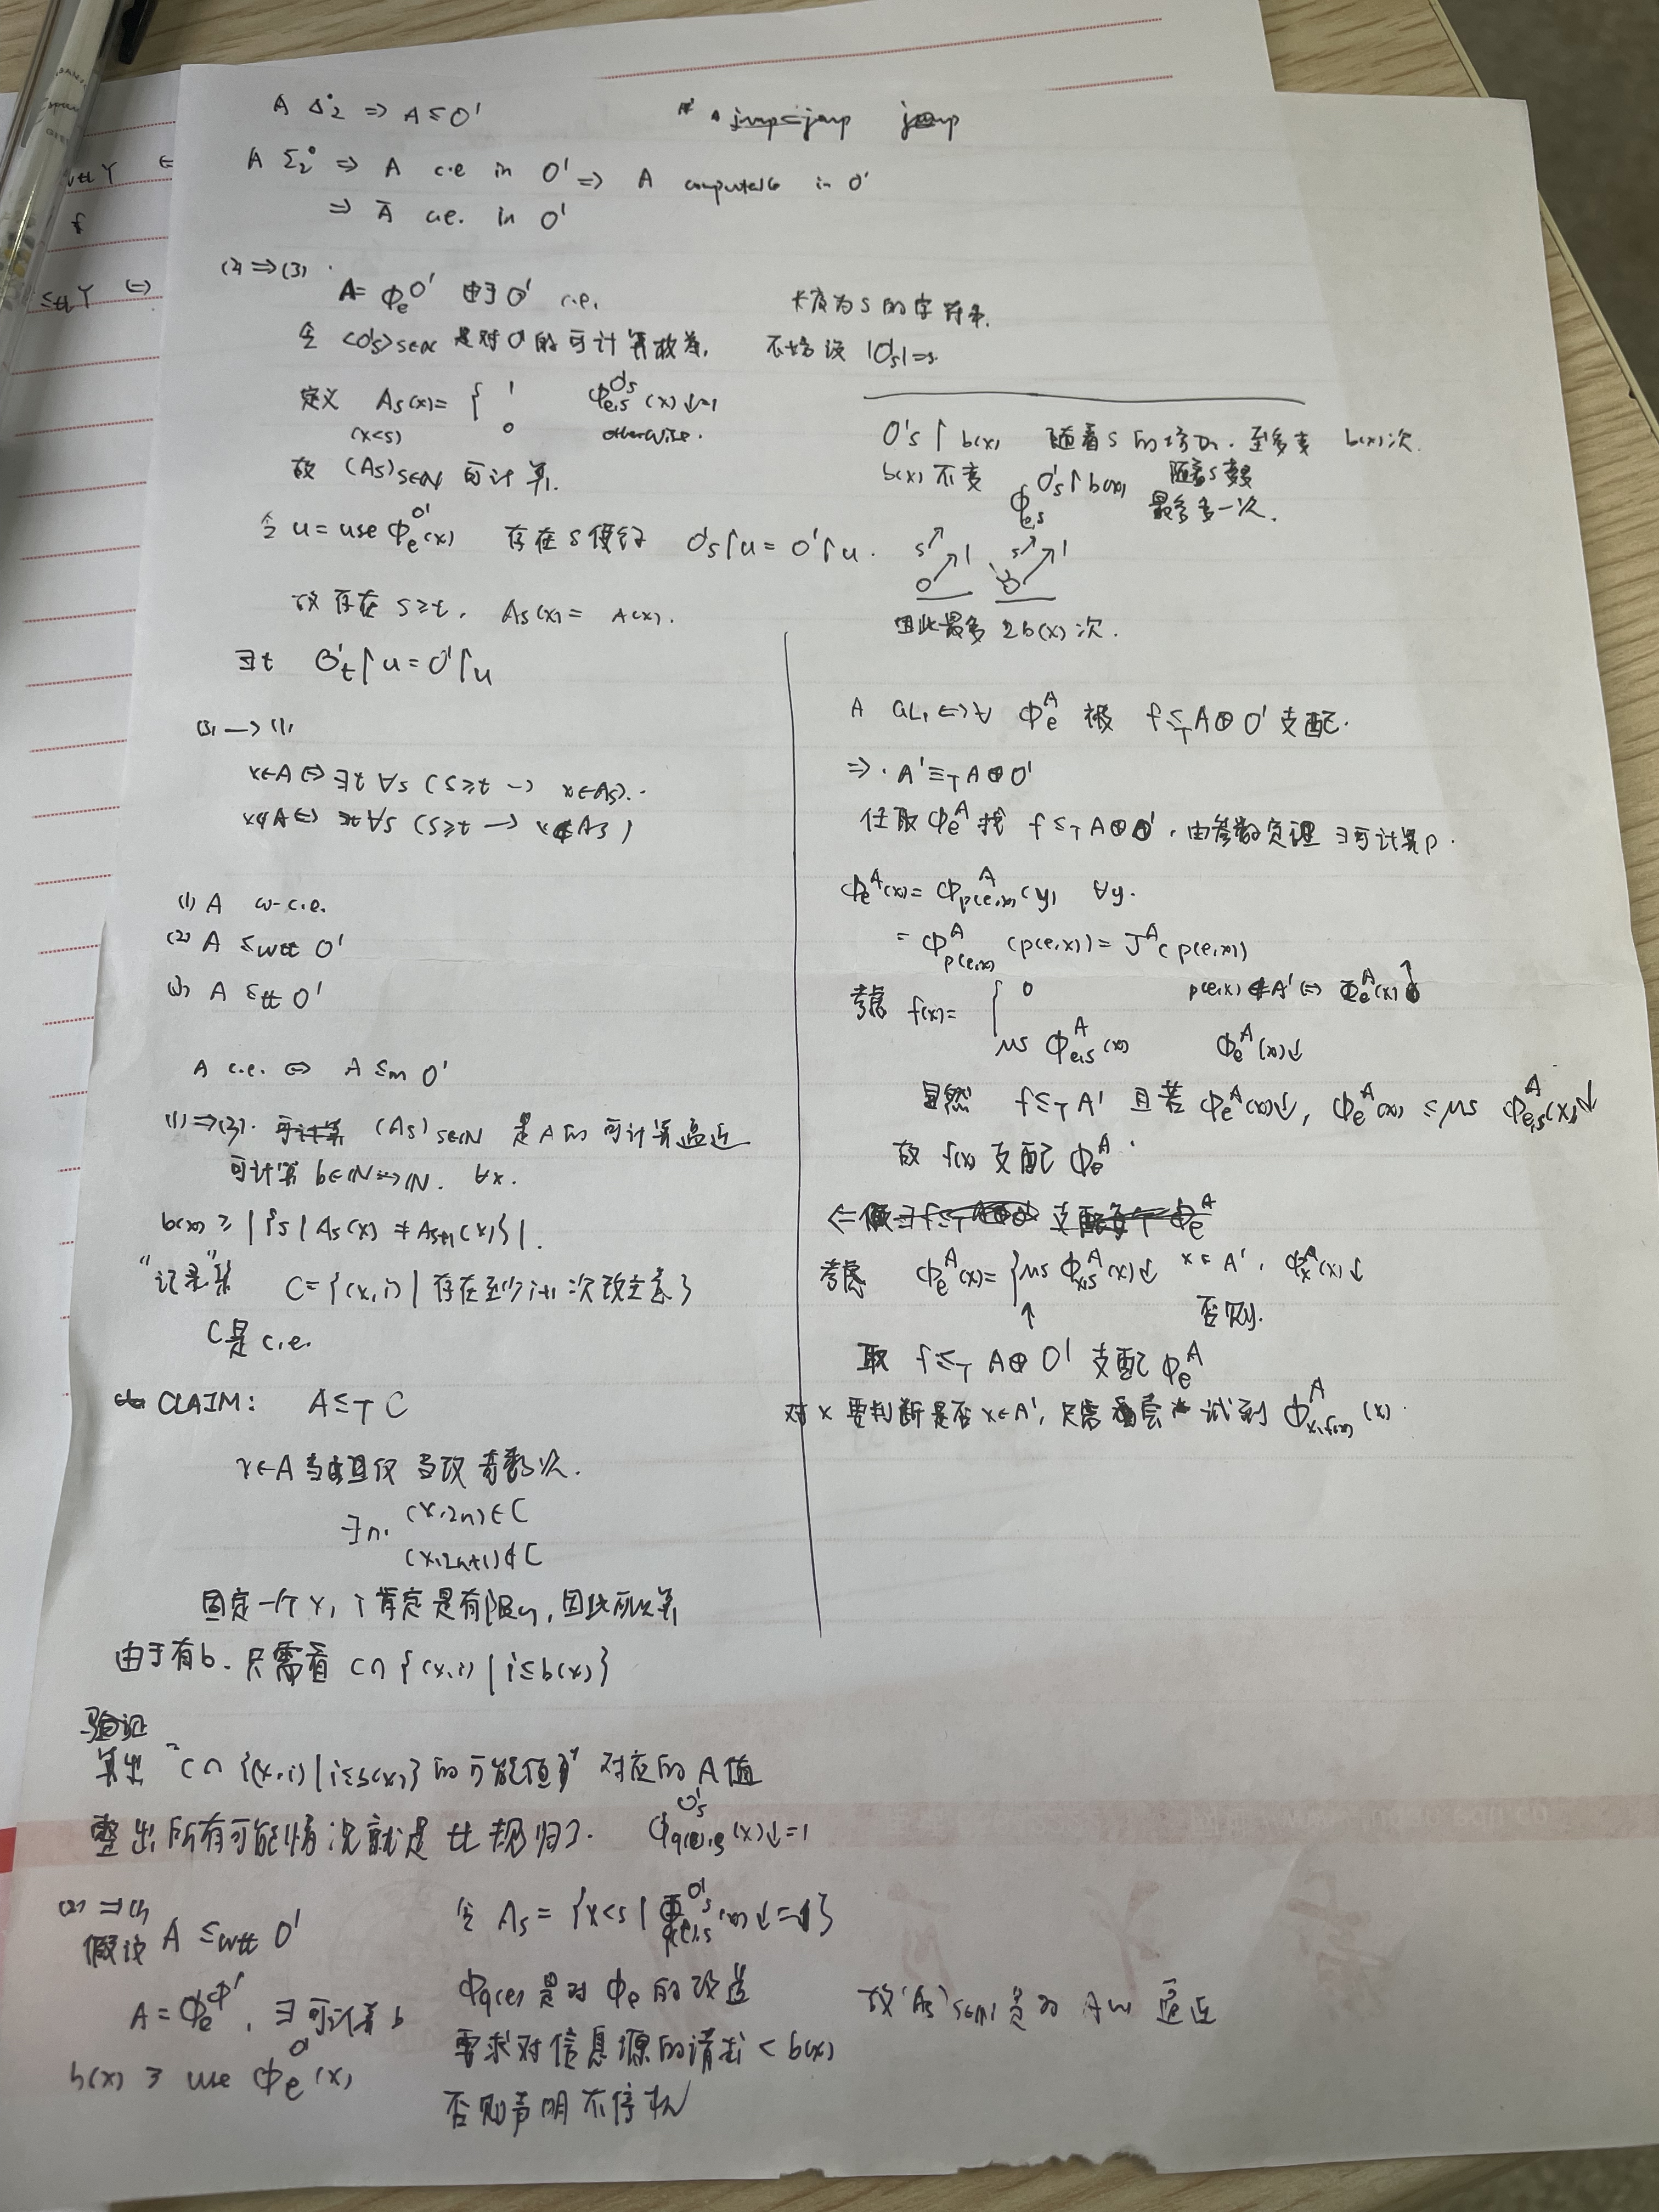
\includegraphics[width=.7\textwidth]{../images/TheRustBook/1.png}
\label{}
\end{figure}

\subsection{References and Borrowing}
\label{sec:orgcfe4829}
\subsection{The Slice Type}
\label{sec:org320002b}
\section{Using Structs to Structure Related Data}
\label{sec:orgdf110ab}
\subsection{Defining and Instantiating Structs}
\label{sec:orgf1f6be2}
\subsection{An Example Program Using Structs}
\label{sec:org67e7ee8}
\end{document}
